\documentclass{beamer}

\usetheme{JuanLesPins}
\usecolortheme{seahorse}

\usepackage[utf8]{inputenc}
\usepackage[T1]{fontenc}
\usepackage{graphicx}
\usepackage{hyperref}
\usepackage{amsmath}

\title{Algoritmy odporúčania filmov v Netflix}
\subtitle{\vspace{3mm} Metódy inžinierskej práce 2024/2025}
\author{Yehor Bohuslavskyi}
\institute{Slovenská technická univerzita v Bratislave}
\date{31. október 2024}

\begin{document}

\begin{frame}
    \titlepage
\end{frame}

\begin{frame}{Prehľad}
    \tableofcontents
\end{frame}

\section{Úvod do odporúčacích systémov}

\begin{frame}{Ciel Netflix}
    \begin{itemize}
        \item Cieľom spoločnosti Netflix je použivať» odporúčacie algoritmy na maximalizáciu spokojnosti používateľov.
        \item Presná personalizácia.
        \item Úspech Netflix je do veľkej miery pripisovaný jeho pokročilým odporúčacím algoritmom.
    \end{itemize}
\end{frame}


\begin{frame}
    \frametitle{Prehľad odporúčacieho systému Netflixu}
    \centering
    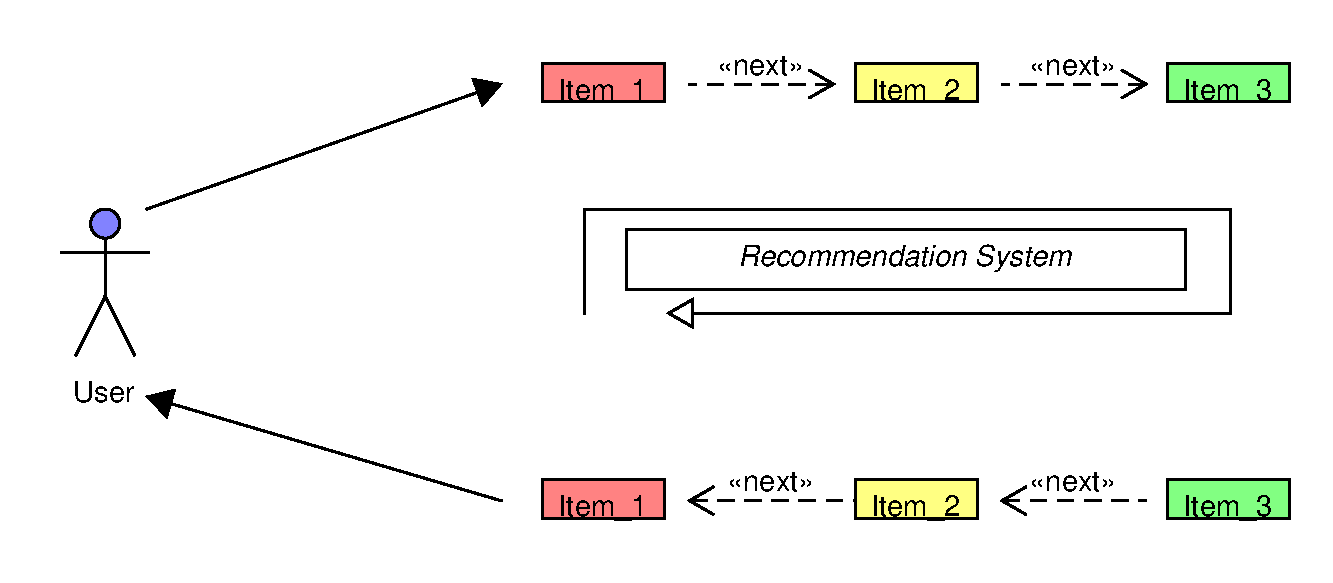
\includegraphics[width=1\textwidth]{Images_tables/RecommendationSystem_pdf.pdf}
    \vspace{1em}
    \textit{image1: Odporúčací systém v Netflixe.}
\end{frame}


\section{Kolaboratívne filtrovanie}

\begin{frame}{Kolaboratívne filtrovanie}
    \begin{itemize}
        \item Predpovedá preferencie porovnaním používateľov s podobným vkusom.
        \item Metódy:
        \begin{itemize}
            \item \textbf{Filtrovanie na základe používateľov:} Odporúča položky, ktoré sa páčili podobným používateľom.
            \item \textbf{Filtrovanie na základe položiek:} Odporúča položky podobné tým, ktoré sa používateľovi páčili.
        \end{itemize}
        \item Výzvy: Problém so studeným štartom, riedkosť dát.
    \end{itemize}
\end{frame}

\section{Filtrovanie na základe obsahu}

\begin{frame}{Filtrovanie na základe obsahu}
    \begin{itemize}
        \item Odporúča položky podobné tým, s ktorými používateľ interagoval.
        \item Založené na atribútoch položiek (žáner, režisér, herci, atď.).
        \item Výhoda: Funguje dobre s novými položkami.
        \item Nevýhoda: Má problém odporúčať rôznorodý obsah.
    \end{itemize}
\end{frame}

\begin{frame}
    \frametitle{Prehľad odporúčacieho systému Netflixu}
    \centering
    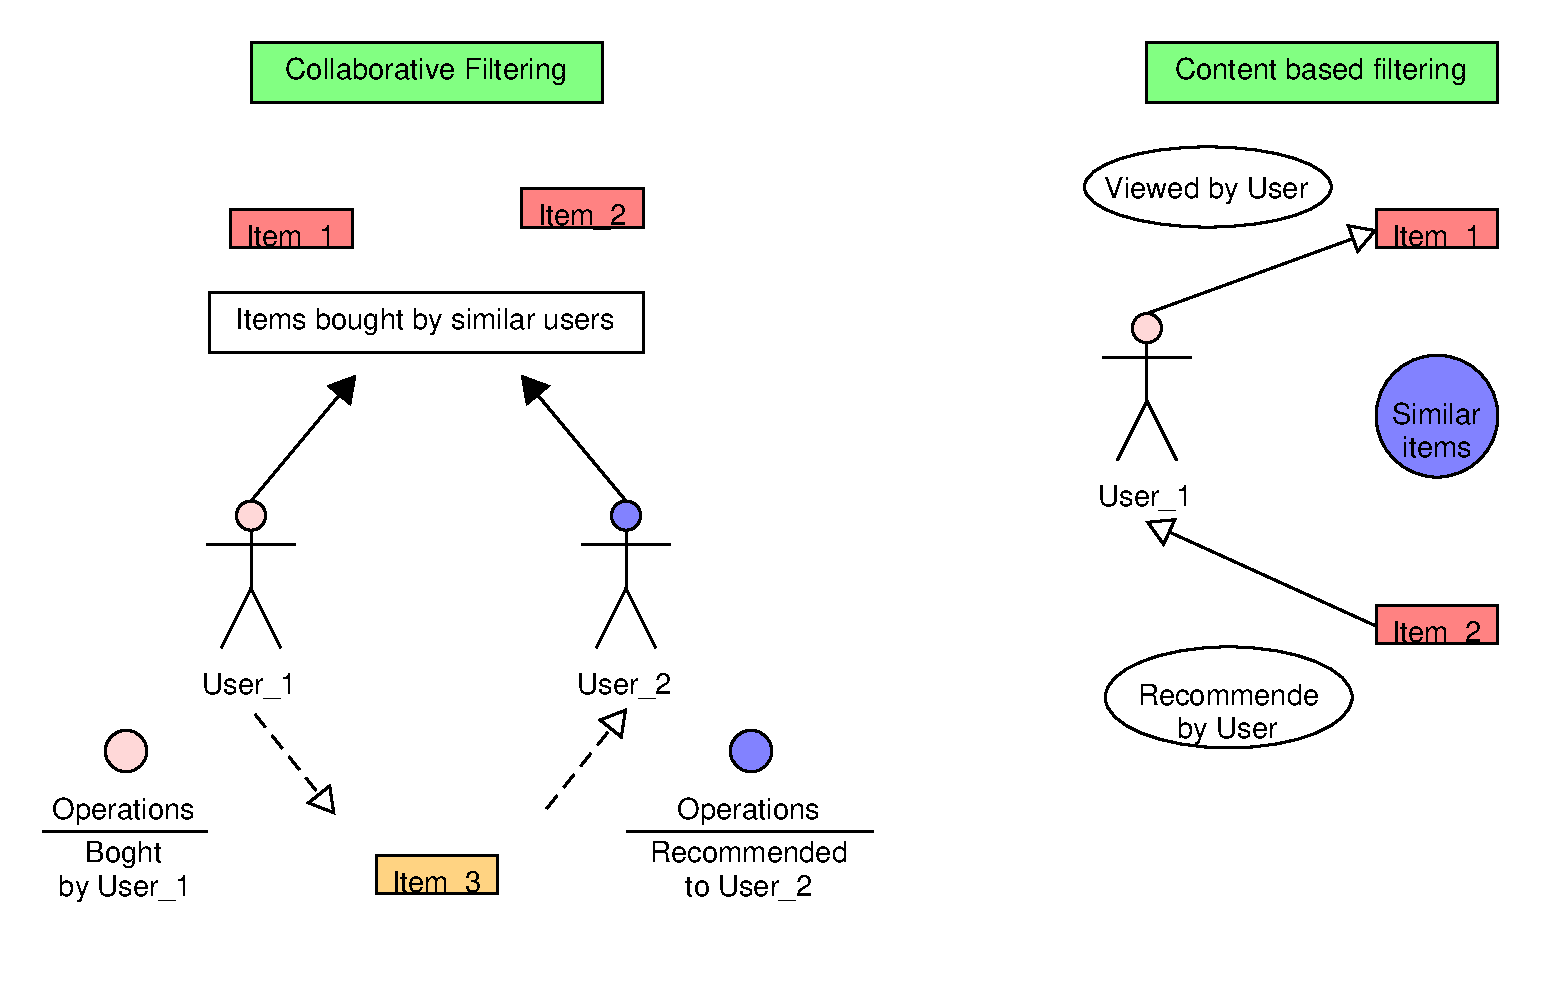
\includegraphics[width=0.9\textwidth]{Images_tables/Filtering_pdf.pdf}
    \vspace{1em}
    \textit{image2: Filtrovanie v Netflix.}
\end{frame}

\section{Umelá inteligencia v Netflixe}

\begin{frame}{Umelá inteligencia v Netflixe}
    \begin{itemize}
        \item Aktívne využívanie umelej inteligencii na zlepšenie presnosti a efektívnosti odporúčania.
        \item Ensemble Learning.
    \end{itemize}
\end{frame}

\section{Ranking}

\begin{frame}{Types of ranking}
    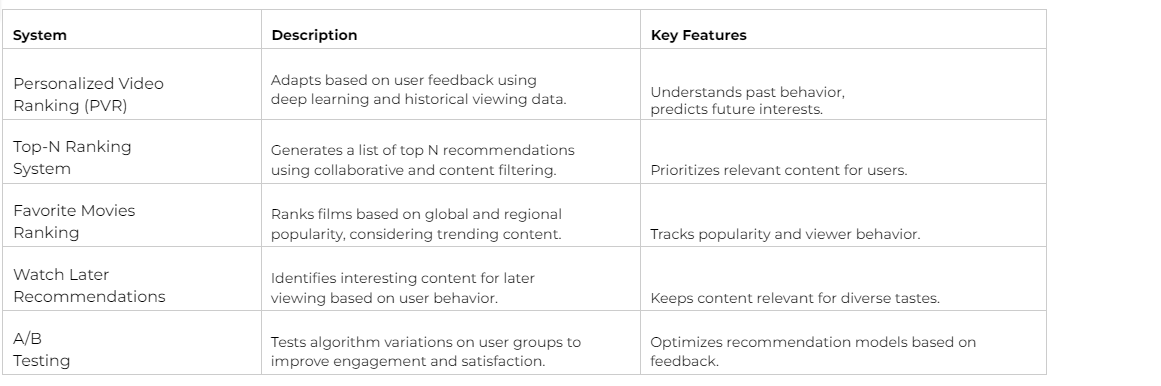
\includegraphics[scale=0.5]{Images_tables/table.png}
\end{frame}

\section{Diagram: Odporúčací pracovný tok}

\section{Záver}

\begin{frame}{Záver}
    \begin{itemize}
        \item Netflix používa hybridný odporúčací systém na poskytovanie personalizovaného obsahu.
        \item Neustále zlepšuje svoje algoritmy, aby zlepšil používateľský zážitok.
        \item Budúce smery: Riešenie problému studeného štartu, zvýšenie rôznorodosti odporúčaní.
    \end{itemize}
\end{frame}

\end{document}
